
%% bare_conf.tex
%% V1.3
%% 2007/01/11
%% by Michael Shell
%% See:
%% http://www.michaelshell.org/
%% for current contact information.
%%
%% This is a skeleton file demonstrating the use of IEEEtran.cls
%% (requires IEEEtran.cls version 1.7 or later) with an IEEE conference paper.
%% Support sites:
%% http://www.michaelshell.org/tex/ieeetran/
%% http://www.ctan.org/tex-archive/macros/latex/contrib/IEEEtran/
%% and
%% http://www.ieee.org/

%%*************************************************************************
%% Legal Notice:
%% This code is offered as-is without any warranty either expressed or
%% implied; without even the implied warranty of MERCHANTABILITY or
%% FITNESS FOR A PARTICULAR PURPOSE! 
%% User assumes all risk.
%% In no event shall IEEE or any contributor to this code be liable for
%% any damages or losses, including, but not limited to, incidental,
%% consequential, or any other damages, resulting from the use or misuse
%% of any information contained here.
%%
%% All comments are the opinions of their respective authors and are not
%% necessarily endorsed by the IEEE.
%%
%% This work is distributed under the LaTeX Project Public License (LPPL)
%% ( http://www.latex-project.org/ ) version 1.3, and may be freely used,
%% distributed and modified. A copy of the LPPL, version 1.3, is included
%% in the base LaTeX documentation of all distributions of LaTeX released
%% 2003/12/01 or later.
%% Retain all contribution notices and credits.
%% ** Modified files should be clearly indicated as such, including  **
%% ** renaming them and changing author support contact information. **
%%
%% File list of work: IEEEtran.cls, IEEEtran_HOWTO.pdf, bare_adv.tex,
%%                    bare_conf.tex, bare_jrnl.tex, bare_jrnl_compsoc.tex
%%*************************************************************************

% *** Authors should verify (and, if needed, correct) their LaTeX system  ***
% *** with the testflow diagnostic prior to trusting their LaTeX platform ***
% *** with production work. IEEE's font choices can trigger bugs that do  ***
% *** not appear when using other class files.                            ***
% The testflow support page is at:
% http://www.michaelshell.org/tex/testflow/



% Note that the a4paper option is mainly intended so that authors in
% countries using A4 can easily print to A4 and see how their papers will
% look in print - the typesetting of the document will not typically be
% affected with changes in paper size (but the bottom and side margins will).
% Use the testflow package mentioned above to verify correct handling of
% both paper sizes by the user's LaTeX system.
%
% Also note that the "draftcls" or "draftclsnofoot", not "draft", option
% should be used if it is desired that the figures are to be displayed in
% draft mode.
%
\documentclass[conference]{IEEEtran}
% Add the compsoc option for Computer Society conferences.
%
% If IEEEtran.cls has not been installed into the LaTeX system files,
% manually specify the path to it like:
% \documentclass[conference]{../sty/IEEEtran}





% Some very useful LaTeX packages include:
% (uncomment the ones you want to load)


% *** MISC UTILITY PACKAGES ***
%
%\usepackage{ifpdf}
% Heiko Oberdiek's ifpdf.sty is very useful if you need conditional
% compilation based on whether the output is pdf or dvi.
% usage:
% \ifpdf
%   % pdf code
% \else
%   % dvi code
% \fi
% The latest version of ifpdf.sty can be obtained from:
% http://www.ctan.org/tex-archive/macros/latex/contrib/oberdiek/
% Also, note that IEEEtran.cls V1.7 and later provides a builtin
% \ifCLASSINFOpdf conditional that works the same way.
% When switching from latex to pdflatex and vice-versa, the compiler may
% have to be run twice to clear warning/error messages.






% *** CITATION PACKAGES ***
%
%\usepackage{cite}
% cite.sty was written by Donald Arseneau
% V1.6 and later of IEEEtran pre-defines the format of the cite.sty package
% \cite{} output to follow that of IEEE. Loading the cite package will
% result in citation numbers being automatically sorted and properly
% "compressed/ranged". e.g., [1], [9], [2], [7], [5], [6] without using
% cite.sty will become [1], [2], [5]--[7], [9] using cite.sty. cite.sty's
% \cite will automatically add leading space, if needed. Use cite.sty's
% noadjust option (cite.sty V3.8 and later) if you want to turn this off.
% cite.sty is already installed on most LaTeX systems. Be sure and use
% version 4.0 (2003-05-27) and later if using hyperref.sty. cite.sty does
% not currently provide for hyperlinked citations.
% The latest version can be obtained at:
% http://www.ctan.org/tex-archive/macros/latex/contrib/cite/
% The documentation is contained in the cite.sty file itself.






% *** GRAPHICS RELATED PACKAGES ***
%
\ifCLASSINFOpdf
  \usepackage[pdftex]{graphicx}
  % declare the path(s) where your graphic files are
  % \graphicspath{{../pdf/}{../jpeg/}}
  % and their extensions so you won't have to specify these with
  % every instance of \includegraphics
  % \DeclareGraphicsExtensions{.pdf,.jpeg,.png}
\else
  % or other class option (dvipsone, dvipdf, if not using dvips). graphicx
  % will default to the driver specified in the system graphics.cfg if no
  % driver is specified.
  % \usepackage[dvips]{graphicx}
  % declare the path(s) where your graphic files are
  % \graphicspath{{../eps/}}
  % and their extensions so you won't have to specify these with
  % every instance of \includegraphics
  % \DeclareGraphicsExtensions{.eps}
\fi
% graphicx was written by David Carlisle and Sebastian Rahtz. It is
% required if you want graphics, photos, etc. graphicx.sty is already
% installed on most LaTeX systems. The latest version and documentation can
% be obtained at: 
% http://www.ctan.org/tex-archive/macros/latex/required/graphics/
% Another good source of documentation is "Using Imported Graphics in
% LaTeX2e" by Keith Reckdahl which can be found as epslatex.ps or
% epslatex.pdf at: http://www.ctan.org/tex-archive/info/
%
% latex, and pdflatex in dvi mode, support graphics in encapsulated
% postscript (.eps) format. pdflatex in pdf mode supports graphics
% in .pdf, .jpeg, .png and .mps (metapost) formats. Users should ensure
% that all non-photo figures use a vector format (.eps, .pdf, .mps) and
% not a bitmapped formats (.jpeg, .png). IEEE frowns on bitmapped formats
% which can result in "jaggedy"/blurry rendering of lines and letters as
% well as large increases in file sizes.
%
% You can find documentation about the pdfTeX application at:
% http://www.tug.org/applications/pdftex





% *** MATH PACKAGES ***
%
%\usepackage[cmex10]{amsmath}
% A popular package from the American Mathematical Society that provides
% many useful and powerful commands for dealing with mathematics. If using
% it, be sure to load this package with the cmex10 option to ensure that
% only type 1 fonts will utilized at all point sizes. Without this option,
% it is possible that some math symbols, particularly those within
% footnotes, will be rendered in bitmap form which will result in a
% document that can not be IEEE Xplore compliant!
%
% Also, note that the amsmath package sets \interdisplaylinepenalty to 10000
% thus preventing page breaks from occurring within multiline equations. Use:
%\interdisplaylinepenalty=2500
% after loading amsmath to restore such page breaks as IEEEtran.cls normally
% does. amsmath.sty is already installed on most LaTeX systems. The latest
% version and documentation can be obtained at:
% http://www.ctan.org/tex-archive/macros/latex/required/amslatex/math/





% *** SPECIALIZED LIST PACKAGES ***
%
%\usepackage{algorithmic}
% algorithmic.sty was written by Peter Williams and Rogerio Brito.
% This package provides an algorithmic environment fo describing algorithms.
% You can use the algorithmic environment in-text or within a figure
% environment to provide for a floating algorithm. Do NOT use the algorithm
% floating environment provided by algorithm.sty (by the same authors) or
% algorithm2e.sty (by Christophe Fiorio) as IEEE does not use dedicated
% algorithm float types and packages that provide these will not provide
% correct IEEE style captions. The latest version and documentation of
% algorithmic.sty can be obtained at:
% http://www.ctan.org/tex-archive/macros/latex/contrib/algorithms/
% There is also a support site at:
% http://algorithms.berlios.de/index.html
% Also of interest may be the (relatively newer and more customizable)
% algorithmicx.sty package by Szasz Janos:
% http://www.ctan.org/tex-archive/macros/latex/contrib/algorithmicx/




% *** ALIGNMENT PACKAGES ***
%
%\usepackage{array}
% Frank Mittelbach's and David Carlisle's array.sty patches and improves
% the standard LaTeX2e array and tabular environments to provide better
% appearance and additional user controls. As the default LaTeX2e table
% generation code is lacking to the point of almost being broken with
% respect to the quality of the end results, all users are strongly
% advised to use an enhanced (at the very least that provided by array.sty)
% set of table tools. array.sty is already installed on most systems. The
% latest version and documentation can be obtained at:
% http://www.ctan.org/tex-archive/macros/latex/required/tools/


%\usepackage{mdwmath}
%\usepackage{mdwtab}
% Also highly recommended is Mark Wooding's extremely powerful MDW tools,
% especially mdwmath.sty and mdwtab.sty which are used to format equations
% and tables, respectively. The MDWtools set is already installed on most
% LaTeX systems. The lastest version and documentation is available at:
% http://www.ctan.org/tex-archive/macros/latex/contrib/mdwtools/


% IEEEtran contains the IEEEeqnarray family of commands that can be used to
% generate multiline equations as well as matrices, tables, etc., of high
% quality.


%\usepackage{eqparbox}
% Also of notable interest is Scott Pakin's eqparbox package for creating
% (automatically sized) equal width boxes - aka "natural width parboxes".
% Available at:
% http://www.ctan.org/tex-archive/macros/latex/contrib/eqparbox/





% *** SUBFIGURE PACKAGES ***
%\usepackage[tight,footnotesize]{subfigure}
% subfigure.sty was written by Steven Douglas Cochran. This package makes it
% easy to put subfigures in your figures. e.g., "Figure 1a and 1b". For IEEE
% work, it is a good idea to load it with the tight package option to reduce
% the amount of white space around the subfigures. subfigure.sty is already
% installed on most LaTeX systems. The latest version and documentation can
% be obtained at:
% http://www.ctan.org/tex-archive/obsolete/macros/latex/contrib/subfigure/
% subfigure.sty has been superceeded by subfig.sty.



%\usepackage[caption=false]{caption}
%\usepackage[font=footnotesize]{subfig}
% subfig.sty, also written by Steven Douglas Cochran, is the modern
% replacement for subfigure.sty. However, subfig.sty requires and
% automatically loads Axel Sommerfeldt's caption.sty which will override
% IEEEtran.cls handling of captions and this will result in nonIEEE style
% figure/table captions. To prevent this problem, be sure and preload
% caption.sty with its "caption=false" package option. This is will preserve
% IEEEtran.cls handing of captions. Version 1.3 (2005/06/28) and later 
% (recommended due to many improvements over 1.2) of subfig.sty supports
% the caption=false option directly:
%\usepackage[caption=false,font=footnotesize]{subfig}
%
% The latest version and documentation can be obtained at:
% http://www.ctan.org/tex-archive/macros/latex/contrib/subfig/
% The latest version and documentation of caption.sty can be obtained at:
% http://www.ctan.org/tex-archive/macros/latex/contrib/caption/




% *** FLOAT PACKAGES ***
%
%\usepackage{fixltx2e}
% fixltx2e, the successor to the earlier fix2col.sty, was written by
% Frank Mittelbach and David Carlisle. This package corrects a few problems
% in the LaTeX2e kernel, the most notable of which is that in current
% LaTeX2e releases, the ordering of single and double column floats is not
% guaranteed to be preserved. Thus, an unpatched LaTeX2e can allow a
% single column figure to be placed prior to an earlier double column
% figure. The latest version and documentation can be found at:
% http://www.ctan.org/tex-archive/macros/latex/base/



%\usepackage{stfloats}
% stfloats.sty was written by Sigitas Tolusis. This package gives LaTeX2e
% the ability to do double column floats at the bottom of the page as well
% as the top. (e.g., "\begin{figure*}[!b]" is not normally possible in
% LaTeX2e). It also provides a command:
%\fnbelowfloat
% to enable the placement of footnotes below bottom floats (the standard
% LaTeX2e kernel puts them above bottom floats). This is an invasive package
% which rewrites many portions of the LaTeX2e float routines. It may not work
% with other packages that modify the LaTeX2e float routines. The latest
% version and documentation can be obtained at:
% http://www.ctan.org/tex-archive/macros/latex/contrib/sttools/
% Documentation is contained in the stfloats.sty comments as well as in the
% presfull.pdf file. Do not use the stfloats baselinefloat ability as IEEE
% does not allow \baselineskip to stretch. Authors submitting work to the
% IEEE should note that IEEE rarely uses double column equations and
% that authors should try to avoid such use. Do not be tempted to use the
% cuted.sty or midfloat.sty packages (also by Sigitas Tolusis) as IEEE does
% not format its papers in such ways.





% *** PDF, URL AND HYPERLINK PACKAGES ***
%
%\usepackage{url}
% url.sty was written by Donald Arseneau. It provides better support for
% handling and breaking URLs. url.sty is already installed on most LaTeX
% systems. The latest version can be obtained at:
% http://www.ctan.org/tex-archive/macros/latex/contrib/misc/
% Read the url.sty source comments for usage information. Basically,
% \url{my_url_here}.





% *** Do not adjust lengths that control margins, column widths, etc. ***
% *** Do not use packages that alter fonts (such as pslatex).         ***
% There should be no need to do such things with IEEEtran.cls V1.6 and later.
% (Unless specifically asked to do so by the journal or conference you plan
% to submit to, of course. )


% correct bad hyphenation here
\hyphenation{op-tical net-works semi-conduc-tor}


\begin{document}
%
% paper title
% can use linebreaks \\ within to get better formatting as desired
\title{Birmingham Autonomous Robot Club (BARC) - Team Description Paper}


% author names and affiliations
% use a multiple column layout for up to three different
% affiliations
\author{\IEEEauthorblockN{Lenka Mudrova, Marco Becerra, Manolis Chiou, Sean Bastable}
\IEEEauthorblockA{
School of Computer Science, University of Birmingham, UK}
%\and
%\IEEEauthorblockN{Ashish Kumar}
%\IEEEauthorblockA{axk380@cs.bham.ac.uk}
%\and
%\IEEEauthorblockN{}
%\IEEEauthorblockA{@cs.bham.ac.uk}
}

% conference papers do not typically use \thanks and this command
% is locked out in conference mode. If really needed, such as for
% the acknowledgment of grants, issue a \IEEEoverridecommandlockouts
% after \documentclass

% for over three affiliations, or if they all won't fit within the width
% of the page, use this alternative format:
% 
%\author{\IEEEauthorblockN{Michael Shell\IEEEauthorrefmark{1},
%Homer Simpson\IEEEauthorrefmark{2},
%James Kirk\IEEEauthorrefmark{3}, 
%Montgomery Scott\IEEEauthorrefmark{3} and
%Eldon Tyrell\IEEEauthorrefmark{4}}
%\IEEEauthorblockA{\IEEEauthorrefmark{1}School of Electrical and Computer Engineering\\
%Georgia Institute of Technology,
%Atlanta, Georgia 30332--0250\\ Email: see http://www.michaelshell.org/contact.html}
%\IEEEauthorblockA{\IEEEauthorrefmark{2}Twentieth Century Fox, Springfield, USA\\
%Email: homer@thesimpsons.com}
%\IEEEauthorblockA{\IEEEauthorrefmark{3}Starfleet Academy, San Francisco, California 96678-2391\\
%Telephone: (800) 555--1212, Fax: (888) 555--1212}
%\IEEEauthorblockA{\IEEEauthorrefmark{4}Tyrell Inc., 123 Replicant Street, Los Angeles, California 90210--4321}}




% use for special paper notices
%\IEEEspecialpapernotice{(Invited Paper)}




% make the title area
\maketitle

\begin{abstract}
%\boldmath
Robotic competitions provide an excellent opportunity for students to use their knowledge and skills from formal lectures and research to real world challenging scenarios. Moreover, they can influence and promote robotics to the public. Experience and knowledge gained from these events pushes research into progressing faster and benefits the robotics community.
Birmingham Autonomous Robot Club (BARC) aims in connecting the students from the School of Computer Science, University of Birmingham, with strong motivation in robotic applications and competitions. This paper is part of our application for participating in the RoCKIn 2014 competition. It provides an overview of our team, including team members, description of their research interests and previous experiences. Also, it provides information on the team's robot and the hardware that will be used. Lastly, it is described in detail how the competition's tasks will be tackled by the team and the software implementation/architecture that it is currently used.
\end{abstract}
% IEEEtran.cls defaults to using nonbold math in the Abstract.
% This preserves the distinction between vectors and scalars. However,
% if the conference you are submitting to favors bold math in the abstract,
% then you can use LaTeX's standard command \boldmath at the very start
% of the abstract to achieve this. Many IEEE journals/conferences frown on
% math in the abstract anyway.

% no keywords




% For peer review papers, you can put extra information on the cover
% page as needed:
% \ifCLASSOPTIONpeerreview
% \begin{center} \bfseries EDICS Category: 3-BBND \end{center}
% \fi
%
% For peerreview papers, this IEEEtran command inserts a page break and
% creates the second title. It will be ignored for other modes.
\IEEEpeerreviewmaketitle



\section{Introduction}
% no \IEEEPARstart

BARC team was established five years ago in the School of Computer Science at the University of Birmingham. The main purpose was to provide an extra opportunity for students to get more knowledge about robotics and to work on real robotic platforms and projects. Students were familiarising themselves with the Robot Operating System (ROS), by using a variety of ROS libraries and packages. Also, they had the chance to work with different robotics platforms.

Several students involved in the team were solving more complicated projects, mainly useful to promote robotics during school's Open day. Such an example was a robot Waitress, that was accepting orders for drinks and was bringing them to the person. This robot had no manipulation, drinks were placed on the robot by a person. Another example can be a project with a Nao robot repeating gestures of kids. An extra Kinect sensor was used to recognize children's gestures. In spite of these interesting projects a lot of students involved in previous years in the club had no real goal and no real deadlines, thus they did not produced any comprehensive work.

This year, the BARC structure was changed in order to incorporate the lessons learned and to allow the team to take part in a robotics competition. We would like to join RoCKIn@home 2014 competition because it provides an interesting challenge and will help progressing domestic and industrial robots research and applications. Moreover, the cooperation between students is necessary. As a result, students can learn how to work in a team, but still work on some challenging part alone and gaining valuable knowledge while learning how to be responsible for their work.

The team has the support of the Intelligent Robotic Lab (cite site here) in the school of Computer Science. The lab conducts research and has expertise in a variety of fields such as but not limited to computer vision, manipulation, planning, architectures, reasoning and mobile robots. Furthermore the lab has strong links with the industry. 

 
\section{Our focus and plan}
%from rules: Innovative technology (if any) TODO describe usage of STRANDS
%from rules: Reusability of the system or parts thereof - see STRANDS
(I think we should mainly focus on re-usability and the chance to produce a complete robotic platform by on state of the art and proven AI for real world applications. )
The team would like to join RoCKIn@Home competition, but the exact rules are not provided yet. Thus, we took a rules of the Robocup@Home challenge and we agree that we will focus on \textit{Follow me} and \textit{Cocktail party} tasks first. We discus the architecture of your system using the Dora robot, see Section \ref{sec:dora}.



\section{Team members}
%from rules:  Main involved research areas in the team work

Currently all team members are students in the School of Computer Science, University of Birmingham. The overview of team members follows along with a description of their background and research interests. The final team line-up is likely to change until the competition as more members will contribute.

\subsection{Lenka Mudrova}

Her role in the team is mainly team leader. She is doing the organization work, such as reports from regular meetings, website presentation and communication with the school about support. She is also a technical manager, this means that she is meeting with single groups solving a particular robot module and try to understand briefly all the system. As a result, she is creating a bridge between the groups and she takes care that everyone knows what is happening and how the modules will communicate and so on. Instead of this, she is working on the robot controller.

\subsubsection*{Scientific background}
Her previous background is also in the robotics, mainly focus on localization of robots. She was involved as a team leader of student robotic team before in the Czech Republic, as you can see from her CV sent as a separate file.

Nowadays, she is a PhD student with the focus on robotics. Her PhD thesis topic is "Cognitive control framework for long-term autonomy". Broadly speaking, the goal her thesis is to create a collection of functions to schedule and plan tasks for a robot that will exploit long-term experiences and observations. Her work is influenced by the EU STRANDS project (http://strands-project.eu/). Citating from the project’s abstract: "STRANDS aims to enable a robot to achieve robust and intelligent behaviour in human environments through adaptation to, and the exploitation of, long-term experience (at least 120 days by the end of the project)."

Currently, she is working on a scheduling system that will be used in the first year of the project. This system will be based on state-of-the-art schedulers. Each input task is defined by a time window when it needs to be executed, expected duration and where in the environment the task should be performed. The scheduler will then output an ordering for the list of input tasks. It also will handle "on-demand" tasks, thus it will also include a rescheduling procedure for when a new task arrives.

Afterwards, she will extend this approach so that the scheduler can tackle other common issues that arise in the robotics domain – e.g., uncertainty about time duration of task, errors occurring during the execution of the task and so on. Also, she will add a planning approach and integrate it with the scheduler, so that more efficient scheduling of tasks can be achieved. In particular, she will investigate how different tasks can be mixed or executed in parallel, instead of the sequential execution usually present in state-of-the-art schedulers.

\subsection{Sean Bastable}

He is an undergraduate student in the Computer Science but with focus on robotics. As he was also a BARC member the previous year, he has experience with ROS and different robotic platforms. ((******He is one of the two people working on a visual tracking system, using the skeleton body recognition and colour information. He is also interested in computer vision, thus the RoCKin camp will be beneficial for him.****)) <- plz update this part.

\subsubsection*{Scientific background}
 
 His final year project is about investigating and implementing a visual localization system for a mobile robot. This will allow the robot to continue localising in environments where laser based localisation cannot be used. A good example of this, are domestic environments where the presence of people moving around the robot may obstruct the laser scan and provide false readings.
 
The project will involve mounting a ceiling facing omnidirectional camera on the top of a robot in order to take pictures of its surroundings.
The robot will be trained by taking many pictures of the environment, along with location data provided through laser based localisation under ideal conditions. When localising, it can then take additional pictures and compare them to the training images in order to find an estimate of its location. He will primarily be using Principal Components Analysis (PCA) to match images in the localisation phase to those in the test phase. The planing of his project also involves investigating other techniques and methods to improve the robustness of the system.

Another potential use of this is to provide an initial location estimate to a laser based localisation system in order to allow the robot to quickly localise from any position without any human input.

This project follows on his Summer project working on a drinks serving robot for a launch event for the 2014 British Science Festival. One of the key failure points was if the robot became de-localised. It needs to know exactly where it is in order to effectively navigate through gaps in between crowds of people, but the crowds make this much more difficult. Visual localisation was considered as a potential solution but would have taken too long to implement.

\subsection{Manolis Chiou}

He is a PhD student in the Intelligent robotics lab of School of Computer Science, University of Birmingham. He has a multidisciplinary background with hands on work on robots and AI. His work on BARC involves but is not limited to navigation, localization and in the future Human-Robot-Interaction (HRI) and different controllers.

\subsubsection*{Scientific background}

His first degree is in Control Engineering from the Technological Institute of Piraeus, in which he got involved in many robotic projects including demonstrating these projects to the public and exhibitions. His undergraduate thesis was on implementing control algorithms to robots (e.g. Model Predictive Control for stability/balance on moving platforms). He has a MSc in Computational Intelligence with his master thesis be on formation and transportation of objects with a swarm of robots.  

The title of his PhD thesis is ``Flexible robotic control via co-operation between an Operator and an AI based control system". It addresses the problem of variable autonomy in teleoperated mobile robots. Variable autonomy refers to the different levels of autonomous capabilities that are implemented on a robot. Robots used on demanding and safety critical tasks (e.g. search and rescue, hazardous environments inspection, bomb disposal), which are currently teleoperated, could soon start to benefit from autonomous capabilities, such as algorithms for automatic robot navigation or algorithms for SLAM. Robots could usefully use AI control algorithms to autonomously take control of certain functions when the human operator is suffering a high workload, high cognitive load, anxiety, or other distractions and stresses. In contrast, some circumstances may still necessitate direct human control of the robot.

The research will tackle the problem by designing a mixed-initiative control algorithm for switching between the different autonomy levels in an optimal way. Mixed-initiative refers to the peer-to-peer relationship between the robot and the operator in terms of the authority to initiate actions and changes in the autonomy level. Research will be conducted and evaluated in a principled way by designing experiments with methods drawn from human factors, psychology, Human-Robot-Interaction and robotics. Lastly, State of the art AI algorithms (e.g. SLAM, navigation etc.) will be implemented on ROS and tested for improving the performance of this variable autonomy - mixed initiative framework.


\section{Hardware}
%TODO change it and enlarge it
%from rules: Description of the hardware, including an image of the robot(s)
The robot Dora (a pioneer robot) was kindly given for the team's needs. Furthermore, team members have access to different sensors such as laser scanners and depth cameras. At the moment Dora has no manipulator arm installed. In the future it is planned to mount one small manipulator arm in order to extent Dora's capabilities and allow for participation in more challenging scenarios in future competitions.

Dora robot (see Fig.\ref{fig:dora}) is a Pioneer 3D-X robotic platform with a Hokuyo laser scanner in the front and a Kinect depth camera mounted on a pan-tilt unit. It is placed on the stick to get snapshot from better heigh than just place it on the Pioneer robot. Dora has also a travel luggage kit, thus it is possible to take her to the competition.


\begin{figure}[!t]
\centering
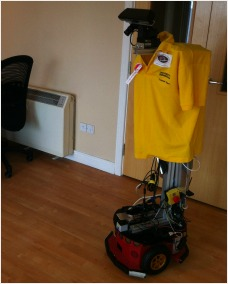
\includegraphics[width=2.in]{dorafinal.jpg}
% where an .eps filename suffix will be assumed under latex, 
% and a .pdf suffix will be assumed for pdflatex; or what has been declared
% via \DeclareGraphicsExtensions.
\caption{Dora robot}
\label{fig:dora}
\end{figure}

\section{Software architecture}
The system is composed of several independent programs/nodes and thus reusable parts of code with different functionality.  The different nodes communicate between them by exchanging ROS messages and ROS actions. The core element of our framework that binds the rest of the node/processes together is a state machine node. (needs heavy editing this part)

\subsection{Middleware-Robot Operating System}
Robot Operating System (ROS) (cite here) will be used as the middleware. ROS open source philosophy is powerful and allows code re-usability by different programmers. It allows us to use robust, state of the art or our own AI algorithms without worrying about how to write code for low level motor commands or sensor drivers. Even more important is the fact that can save valuable time that otherwise would be spend in merging different architectures or worrying of how different pieces of software would communicate with each other. Lastly, ROS was also chosen as it has become almost a standard choice for researchers and thus our lab has extensive hands on experience.

\subsection{State machine}
The core element of our framework that binds the rest of the node/processes together is a state machine node. It is responsible for monitoring the state of the robot and the world. Also it is responsible for deciding what is going to be the next robot action. It was developed with ROS SMACH framework and it works by....

\subsection{Building the map with SLAM}
Since the map is it assumed to be known there is a need to build it before further tests can be done. For initially building a map we made use of the OpenSlam's Gmapping algorithm (citation) through the ROS wrapper package slam gmapping. It uses bla bla...

\subsection{Localising in a known map with adaptive Monte Carlo localisation}
After the map is known and saved, Adaptive Monte Carlo Localisation (AMCL) algorithm (is part of the ROS navigation stack - see next section) is used to localise the robot inside the environment. It uses robot odometry and laser range finder readings to update a particle filter that is representing the uncertainty of robot's position within the known map. The robot's pose estimate is then published through a ROS topic...

\subsection{Navigation}
For navigation and obstacle avoidance, ROS navigation stack is used. It is a proven robust solution for domestic environments (citation here of marathon). More specifically navigation stack reads the odometry, the pose estimate and laser range finder scans from the relevant topics and drives safety the robot inside the environment to some goal. The goal is represented by some given coordinates. For example it drives the robot to the door coordinates, where the robot should perform its face recognition to the person ringing the bell. For achiving this it make use of a global and a local planer. The global planner creates an optimal global path based on robot's pose and a global costmap. Then a local planner, making use of the Dynamic Window Approach algorithm (citation here), is responsible for following that global path and reactively avoiding obstacles.

\subsection{Mixed initiative controller and teleoperation}
These nodes were made as part of another project involving mixed initiative Human-Robot Interaction (HRI) in emergency response robots. Thus, the name is not representative of their exact functionality in this case. The controller it is used to decide which velocity commands to give to the motors whenever some coupling of commands is needed. On one hand are the motor commands coming from robot's AI (e.g. AI navigation) and on the other hand are motor commands coming from a teleoperation node and a human through a joystick. Although the robot is autonomous, the latter is necessary as the user needs to place the robot in the initial state, move it around during testing just by pausing AI commands, or stop the robot in the case of an emergency (e.g. robot repeatedly hitting a wall, so the user has to stop it and drive it away).  This is another example of code which can be reused in many different applications.

\subsection{Dora navigation goals node}
\subsection{Face recognition}
\subsection{Transformations}

\section{Future work}
%and maybe enlargements?
%from rules: Applicability and relevance to domestic/industrial robotics [@Home / @Work]


% An example of a floating figure using the graphicx package.
% Note that \label must occur AFTER (or within) \caption.
% For figures, \caption should occur after the \includegraphics.
% Note that IEEEtran v1.7 and later has special internal code that
% is designed to preserve the operation of \label within \caption
% even when the captionsoff option is in effect. However, because
% of issues like this, it may be the safest practice to put all your
% \label just after \caption rather than within \caption{}.
%
% Reminder: the "draftcls" or "draftclsnofoot", not "draft", class
% option should be used if it is desired that the figures are to be
% displayed while in draft mode.
%
%\begin{figure}[!t]
%\centering
%\includegraphics[width=2.5in]{myfigure}
% where an .eps filename suffix will be assumed under latex, 
% and a .pdf suffix will be assumed for pdflatex; or what has been declared
% via \DeclareGraphicsExtensions.
%\caption{Simulation Results}
%\label{fig_sim}
%\end{figure}

% Note that IEEE typically puts floats only at the top, even when this
% results in a large percentage of a column being occupied by floats.


% An example of a double column floating figure using two subfigures.
% (The subfig.sty package must be loaded for this to work.)
% The subfigure \label commands are set within each subfloat command, the
% \label for the overall figure must come after \caption.
% \hfil must be used as a separator to get equal spacing.
% The subfigure.sty package works much the same way, except \subfigure is
% used instead of \subfloat.
%
%\begin{figure*}[!t]
%\centerline{\subfloat[Case I]\includegraphics[width=2.5in]{subfigcase1}%
%\label{fig_first_case}}
%\hfil
%\subfloat[Case II]{\includegraphics[width=2.5in]{subfigcase2}%
%\label{fig_second_case}}}
%\caption{Simulation results}
%\label{fig_sim}
%\end{figure*}
%
% Note that often IEEE papers with subfigures do not employ subfigure
% captions (using the optional argument to \subfloat), but instead will
% reference/describe all of them (a), (b), etc., within the main caption.


% An example of a floating table. Note that, for IEEE style tables, the 
% \caption command should come BEFORE the table. Table text will default to
% \footnotesize as IEEE normally uses this smaller font for tables.
% The \label must come after \caption as always.
%
%\begin{table}[!t]
%% increase table row spacing, adjust to taste
%\renewcommand{\arraystretch}{1.3}
% if using array.sty, it might be a good idea to tweak the value of
% \extrarowheight as needed to properly center the text within the cells
%\caption{An Example of a Table}
%\label{table_example}
%\centering
%% Some packages, such as MDW tools, offer better commands for making tables
%% than the plain LaTeX2e tabular which is used here.
%\begin{tabular}{|c||c|}
%\hline
%One & Two\\
%\hline
%Three & Four\\
%\hline
%\end{tabular}
%\end{table}


% Note that IEEE does not put floats in the very first column - or typically
% anywhere on the first page for that matter. Also, in-text middle ("here")
% positioning is not used. Most IEEE journals/conferences use top floats
% exclusively. Note that, LaTeX2e, unlike IEEE journals/conferences, places
% footnotes above bottom floats. This can be corrected via the \fnbelowfloat
% command of the stfloats package.



\section{Conclusion}
All team members have a strong motivation in participating in the robotic competitions. We think that the RoCKIn@Home will provide interesting challenge for us and it will address the problematic of the real robots in our homes. As a result, we are expecting to obtain more knowledge in the ongoing research in many fields in robotic.

If three our members will be accepted to participate in the RoCKIn camp, we assumed this will help us to get into the demanding robotic topics more faster and produce better and more interesting solution of the overall system.




% conference papers do not normally have an appendix


% use section* for acknowledgement
%\section*{Acknowledgment}







% trigger a \newpage just before the given reference
% number - used to balance the columns on the last page
% adjust value as needed - may need to be readjusted if
% the document is modified later
%\IEEEtriggeratref{8}
% The "triggered" command can be changed if desired:
%\IEEEtriggercmd{\enlargethispage{-5in}}

% references section

% can use a bibliography generated by BibTeX as a .bbl file
% BibTeX documentation can be easily obtained at:
% http://www.ctan.org/tex-archive/biblio/bibtex/contrib/doc/
% The IEEEtran BibTeX style support page is at:
% http://www.michaelshell.org/tex/ieeetran/bibtex/
%\bibliographystyle{IEEEtran}
% argument is your BibTeX string definitions and bibliography database(s)
%\bibliography{IEEEabrv,../bib/paper}
%
% <OR> manually copy in the resultant .bbl file
% set second argument of \begin to the number of references
% (used to reserve space for the reference number labels box)
%\begin{thebibliography}{1}

%\bibitem{IEEEhowto:kopka}
%H.~Kopka and P.~W. Daly, \emph{A Guide to \LaTeX}, 3rd~ed.\hskip 1em plus
%  0.5em minus 0.4em\relax Harlow, England: Addison-Wesley, 1999.

%\end{thebibliography}




% that's all folks
\end{document}


